\section{Experimental Settings for Chapter~\ref{Chapter: CARS}}\label{appendix: Experiments}
In this Section, we list the hyperparameters we used for each experiment. The code for all experiments can be found in \url{https://github.com/bumsu-kim/CARS}. We ran experiments on several machines to distribute the load. We used Intel i5-9400F with Nvidia RTX 2060 and i9-9940X with two RTX 2080.

\paragraph{Mor\'{e}-Garbow-Hillstrom Problems.}
The Mor\'{e}-Garbow-Hillstrom Problem set consists of 34 non-convex smooth functions, where the problem dimension lies between 2 and 100. This experiment is conducted in Matlab.

We consider a problem solved when $f(x_k) - f_{\star} \leq \varepsilon(f(x_0) - f_\star)$. The target accuracies used here are $\varepsilon = 10^{-1}, 10^{-3}$ and $10^{-5}$.
We used the recommended $x_0$ for each problem.

For CARS and CARS-NQ, we used the sampling radius $r_k = 0.01/\sqrt{k+1}$, $\hat{L} = 2$. For CARS-NQ, the number of quadrature points $q=5$ is used. Having larger $q$ increases the accuracy of the approximation of smoothed derivatives, but it also increases the cost ({\em i.e.} function queries required) at each step. Recall from Section~\ref{section: CARS-NQ} that using odd $q$ is always more efficient than even $q$. Since $q=3$ is essentially less accurate than CARS, we used several values of $q\geq 5$ and found that $q=5$ is the best.

For STP \cite{bergou2020stochastic} and NSRS \cite{nesterov2017random} we used the same hyperparameters as given in Section 8.1 of \cite{bergou2020stochastic}. We also used the same decreasing step-size for Stochastic Momentum Three Points method (SMTP) \cite{gorbunov2019stochastic}. For the momentum parameter $\beta$ for SMTP, we followed \cite{gorbunov2019stochastic} and used $\beta = 0.5$.
Namely, following the notations in \cite{bergou2020stochastic} and \cite{gorbunov2019stochastic},
$\mathcal{D} = \unif {(\mathbb{S}^{d-1})}$ and 
\begin{align}
    \alpha_k & = \frac{1}{\sqrt{k+1}}, \tag{STP}\\
    \alpha_k & = \frac{1}{4(n+4)} \textrm{ and } \mu_k = 10^{-4}, \tag{NSRS}\\
    \gamma_k & = \frac{1}{\sqrt{k+1}}, \textrm{ and } \beta = 0.5. \tag{SMTP}
\end{align}

For SPSA \cite{spall1992multivariate} and 2SPSA \cite{spall2000adaptive}, we used the Rademacher distribution ({\em i.e.} $(u_k)_i = \pm 1$ with probability 0.5) for $\mathcal{D}$,  $\alpha = 0.602$, $\gamma = 0.101$, $A = 100$, $a = 0.16$, and $c = 10^{-4}$.

For AdaDGS \cite{tran2020adadgs}, we used the code provided by the authors, by implementing the original Python code in Matlab. Some modifications on hyperparameters are made due to the difference in the scale of problem dimension, and the lack of domain width. First, the original AdaDGS code performs experiments on high dimensional problems  ({\em e.g.} $d=1000$), whereas $2\leq d \leq 100$ in this experiment. Also, the problems are unconstrained, and $\|x_0-x_{\star}\|$ varies from order of $10^0$ to $10^6$.
Thus we used the following modified hyperparameters (following the notation of \cite{tran2020adadgs}):
\begin{enumerate}
    \item The number of points used for line search $S = 100$, since the suggested value $0.05d(M-1)$ is too small for our experiments.
    \item The initial smoothing(sampling) radius $\sigma_0 = 10^{-2}$. We tested $\sigma_0 = 5, 1, 10^{-1}, 10^{-2}$ and $10^{-3}$ and chose the best value. When $\sigma_0 \leq 10^{-1}$ then the results were similar.
\end{enumerate}

For plotting the performance profile, we set the performance ratio $r_{p,s} = r_{M}$ when $p$ is not solved by $s$. Having $r_M = \infty$ is ideal, but setting it by a sufficiently large number does not make any difference. We used $r_M = 10^{20}$.

\paragraph{Problems with Highly Oscillatory Noise.}
For the presence of oscillatory noise scenario, we performed experiments, by adding the noise to Mor\'{e}-Garbow-Hillstrom Problems.
For each function in the benchmark set, we used the same noise
\begin{equation*}
    f_{\mathrm{osc}}(x) = \psi \sum_{i=1}^{d}(1-\cos(\phi_i x_i)), 
\end{equation*}
with different noise level $\psi = 0.1\varepsilon(f(x_0)-f_\star)$, and the same frequency $\phi_i = 100\pi$.

We used the same hyperparameters for Mor\'{e}-Garbow-Hillstrom Problems as in the previous experiment, except for CARS-NQ, where we used 50 times larger $r$.

\paragraph{Black-box Adversarial Attacks.}
In this section, we explain the experiment setting for black-box adversarial attacks and also provide the hyperparameters that we used.
The CNN model we attack has two $5\times5$ convolutional layers with 6 and 16 output channels, followed by a $4\times 4$ convolutional layer with 120 output channels. Then two fully connected layers with 84 and 10 units follows. Between layers we use ReLU, and between convolutional layers we use $2\times 2$ max-pooling as well. Finally we apply log softmax to the output layer.
The test accuracy of the trained model is 98.99\%.

For more readable description, let the images have width and height both equal to $s$. Then the problem dimension $d$ is $s^2$. For this particular experiment, we make three modifications to CARS.
First, since the problem is highly non-convex ($h_r<0$ at around 50\% of the iteration), we don't compute $x_{\mathrm{CARS}}$ when $h_r < 0$ at $k$-th iteration.
The second modification is due to the constraint of the problem. Let $\mathcal{F}$ be the feasible set:
\begin{equation*}
    \mathcal{F} = \{x \in [0,1]^d : \|x-x_0\| \leq \varepsilon_{\mathrm{atk}} \}.
\end{equation*}
Inspired by \cite{andriushchenko2020square}, we also compute $x_{\mathrm{bdry}} = x_k - t_{\mathrm{max}}d_r u_k$, where
\begin{equation*}
    t_{\mathrm{max}} = \max \{ t > 0 : x_k - td_r u_k \in \mathcal{F}\}.
\end{equation*}
This is especially useful when $h_r < 0$ so we don't compute $x_{\mathrm{CARS}}$.
Therefore, CARS now requires either 3 ($f(x_k \pm r_k u_k)$ and $f(x_{\mathrm{bdry}})$) function queries or 
4 ($f(x_{\mathrm{CARS}})$ in addition) per iteration. To sum up,
\begin{align*}
    x_{k+1} = 
    \begin{cases}
        \argmin\{f(x_k \pm r_k u_k), f(x_{\mathrm{CARS}}), (x_{\mathrm{bdry}}) \} & \textrm{ if } h_r>0 \\
        \argmin\{f(x_k \pm r_k u_k), (x_{\mathrm{bdry}}) \} & \text{ otherwise. }
    \end{cases}
\end{align*}
Lastly, we perturbed $x_0$ by adding horizontal stripes. That is,
\begin{equation*}
    x_0 = \mathrm{proj}_{\mathcal{F}} (x_{\mathrm{orig}} + \varepsilon_{\mathrm{atk}} v),
\end{equation*}
where $v_{i,:} = \pm (1,\cdots,1)$ for $i=1,\cdots,s$ and $x_{\mathrm{orig}}$ is the image to be attacked. This choice of initialization is found to be very effective in \cite{andriushchenko2020square}.

We use the same sampling distribution as Square Attack \cite{andriushchenko2020square}, which is known to be particularly well-suited for attacking CNN models. Identifying $s\times s$ images and $d$-vectors,
this distribution generates a square block of all $1$ or $-1$, {\em i.e.} $u_{r+1:r+w, c+1:c+w} = \pm 1$, where $0 \leq r, c \leq s-w$ and $w$ is the window size. See \cite{andriushchenko2020square} for more details.

The window size $w$ is determined by $p$, the fraction of the pixels changed by attack. Namely, $w$ is the closest positive integer to $\sqrt{p}s$, and thus this $p$ is an important hyperparameter in this distribution.
In \cite{andriushchenko2020square}, the authors used $p = 0.8$ in the initial stage and halve the value of $p$ when the number of iteration $k$ reaches $10, 50, 200, 1000, 2000, 4000, 6000$ and $8000$, respectively.

For CARS, we used the initial $p=0.2$ and halved it at $k = 2, 10, 40, 250, 500, 800, 1200$ and $1600$. Note that the Square Attack only uses one function query at each iteration and CARS for black-box attack uses 3 or 4 queries, and thus $p$ is being halved at similar stage of the algorithms, in terms of the function queries.

Finally, the sampling radius $r_k$ is fixed by 1 for every iteration.

\section{Visualization of Attacked Images}
In this section we present the visualization of the attacked images, comparing them with the original images.
To be more clear, the images in Figure~\ref{fig:MNIST_ATK_RES_ALL} have {\em Testset ID} (TID)'s from 100 to 109.
When an image with label $n$ has TID $t$, this means it is the $t$-th $n$ appearing in the test set. See the code for more details on TID.
\begin{figure}[t]
    \centering
    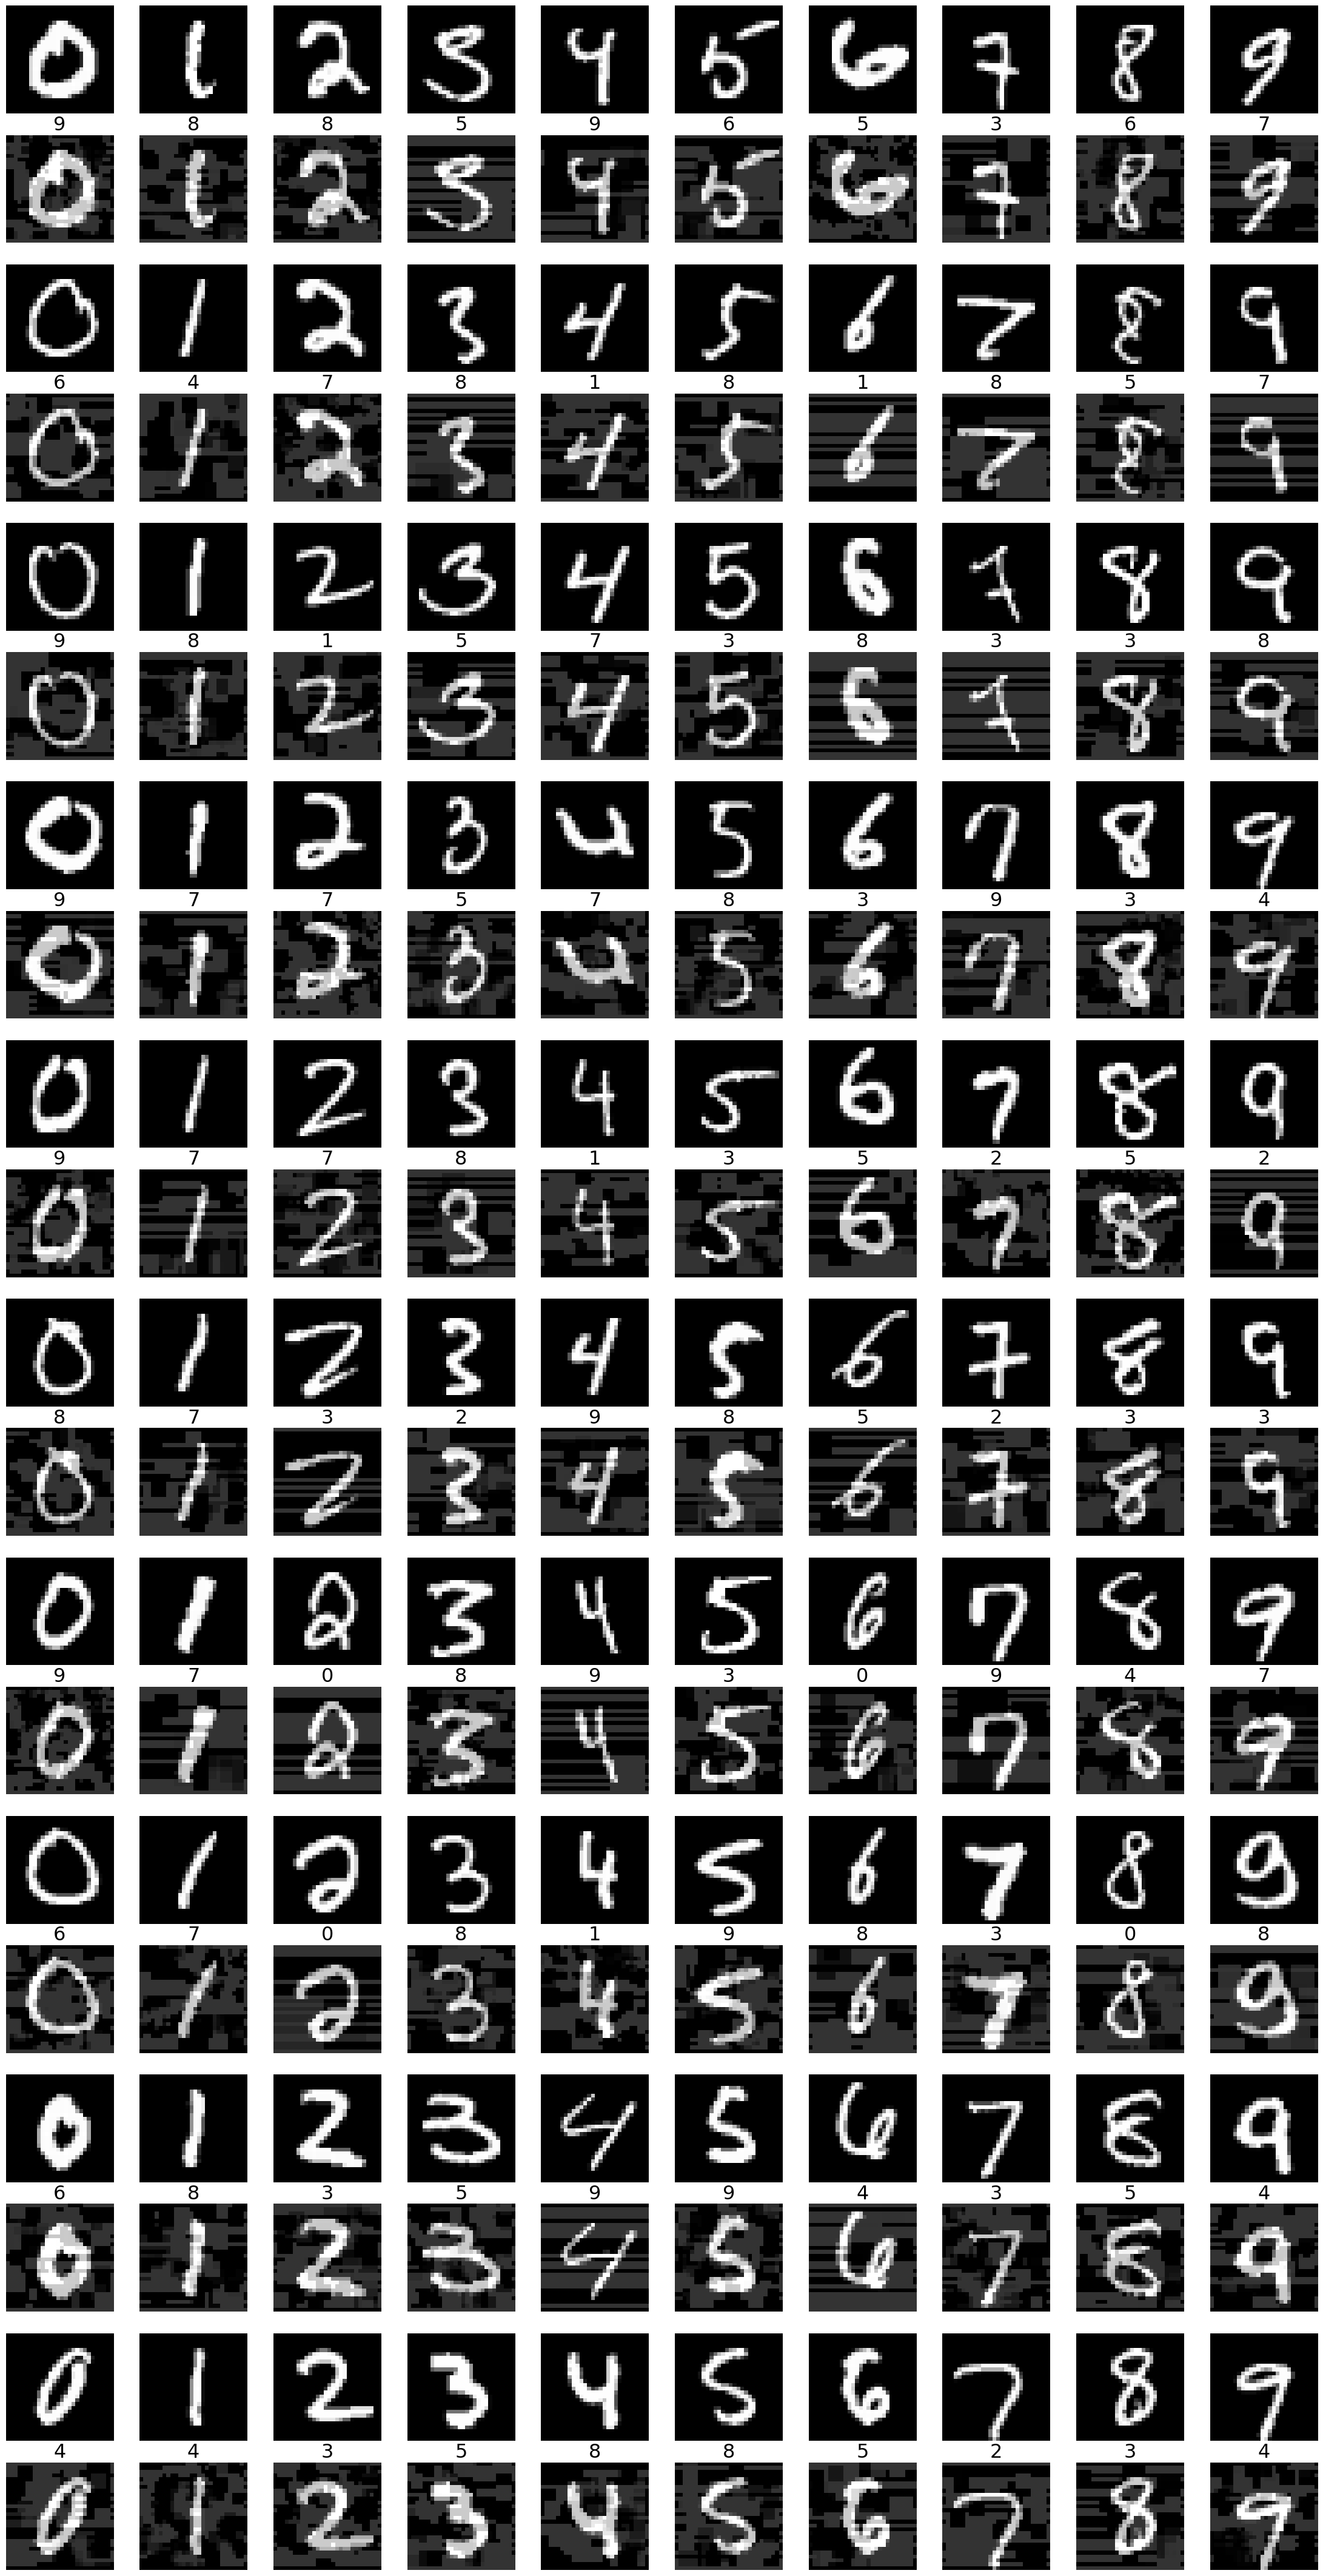
\includegraphics[width=0.60\linewidth]{fig/fig_CARS/MNISTatk_imgs.png}
    \caption{Adversarial examples with misclassified labels on MNIST generated with CARS. For every two rows, a row of original images are shown, and the adversarial examples are right underneath them, with the misclassified labels in between.}
    \label{fig:MNIST_ATK_RES_ALL}
\end{figure}